\chapter{Perancangan}
\label{chap:perancangan}

Bab ini membahas perancangan fitur kolektor pengumuman. Pembahasan dibagi menjadi tiga bagian, yaitu: perancangan kelas, perancangan basis data, dan perancangan antarmuka.
 
\section{Perancangan Kelas}
\begin{figure}[H]
	\centering  
	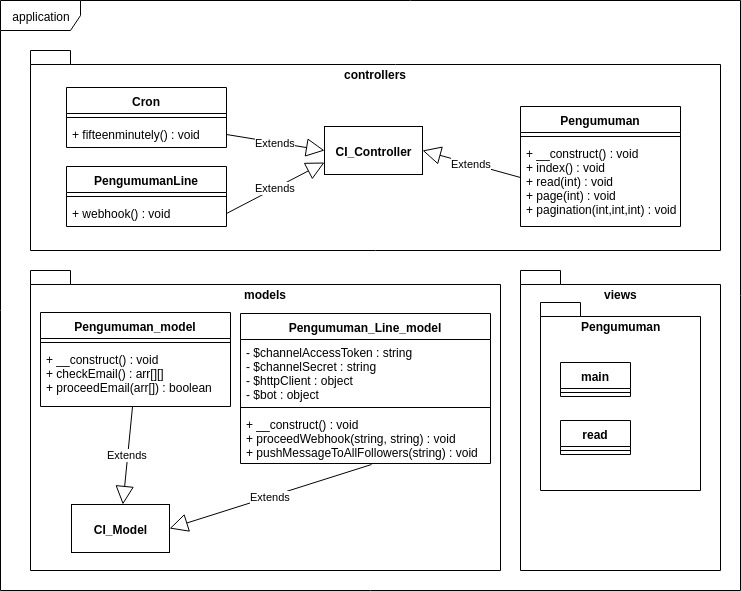
\includegraphics[width=\textwidth]{class-diagram.jpg}  
	\caption[Class diagram fitur kolektor pengumuman]{Class diagram fitur kolektor pengumuman} 
	\label{fig:class-diagram} 
\end{figure}
Gambar~\ref{fig:class-diagram} merupakan gambar diagram kelas yang dipakai untuk pembangunan fitur kolektor pengumuman. Penjelasan untuk diagram kelas tersebut akan diberikan di subbagian. Penjelasan dibagi menjadi tiga bagian: \textit{controller, model, dan view}.

\subsection{Model}
Model yang digunakan ada dua, yaitu Pengumuman\_model dan Pengumuman\_Line\_model.
\subsubsection{Pengumuman\_model}
Pengumuman\_model berisi algoritma yang dibutuhkan oleh fitur kolektor pengumuman. Pengumuman\_model memiliki tiga \textit{method}: \_\_construct, checkEmail, dan proceedEmail. Tabel \ref{table:pengumuman-model-construct}, \ref{table:pengumuman-model-checkemail}, dan \ref{table:pengumuman-model-proceedemail} menjelaskan secara rinci \textit{method-method} tersebut.

\begin{center}
	\begin{table}[H]
	\caption{Rincian method \_\_construct}
	\label{table:pengumuman-model-construct}
\begin{tabular}{|c|p{11cm}|}
\hline
Nama \textit{Method} 	& 	 	\_\_construct \\
\hline
Parameter \textit{Input} & - \\
\hline
Parameter \textit{Output} & - \\
\hline
Tabel yang berhubungan & -\\
\hline
Kelas yang berhubungan &  - \\
\hline
Deskripsi	& \textit{Method} ini digunakan untuk konstruksi\\
\hline
Algoritma	& \begin{enumerate}
				\item Konstruksi dari \textit{parent}.
				\item \textit{Load config auth} dan \textit{modules}.
				\end{enumerate} \\
\hline
\end{tabular}
\end{table}
\end{center}

\begin{center}
	\begin{table}[H]
	\caption{Rincian method checkEmail}
	\label{table:pengumuman-model-checkemail}
\begin{tabular}{|c|p{11cm}|}
\hline
Nama \textit{Method} 	& 	 	checkEmail\\
\hline
Parameter \textit{Input} & - \\
\hline
Parameter \textit{Output} & \textit{Array} dua dimensi. Dimensi pertama mewakili satu \textit{email}, sedangkan dimensi kedua mewakili informasi dari \textit{email} tersebut.\\
\hline
Tabel yang berhubungan & - \\
\hline
Kelas yang berhubungan & - \\
\hline
Deskripsi	& \\
\hline
Algoritma	& \begin{enumerate}
				\item Membuka koneksi IMAP ke \textit{email} pengumuman.
				\item Mencari \textit{email} yang belum dibaca.
				\item Apabila ada \textit{email} yang belum dibaca, maka \textit{email} tersebut dan informasinya dimasukkan ke dalam array.
				\item Menutup koneksi IMAP dan mengembalikan array.
				\end{enumerate} \\
\hline
\end{tabular}
\end{table}
\end{center}

\begin{center}
	\begin{table}[H]
	\caption{Rincian method proceedEmail}
	\label{table:pengumuman-model-proceedemail}
\begin{tabular}{|c|p{11cm}|}
\hline
Nama \textit{Method} 	& 	 proceedEmail	\\
\hline
Parameter \textit{Input} & \textit{Array} asosiatif berisi informasi dari sebuah \textit{email}. \\
\hline
Parameter \textit{Output} & Mengembalikan \textit{true} apabila \textit{email} termasuk \textit{email} pengumuman dan mengembalikan \textit{false} apabila \textit{email} tidak termasuk \textit{email} pengumuman.  \\
\hline
Tabel yang berhubungan & Pengumuman \\
\hline
Kelas yang berhubungan &  Pengumuman\_Line\_model \\
\hline
Deskripsi	& \textit{Method} ini berfungsi untuk memroses \textit{email} pengumuman\\
\hline
Algoritma	& \begin{enumerate}
				\item \textit{Load config} pengumuman
				\item Memeriksa pengirim setiap \textit{email}. Apabila pengirim terdaftar di \textit{config} pengirimTerverifikasi, maka \textit{email} tersebut akan masuk ke tahap berikutnya.
				\item Tahap berikutnya adalah memasukkan informasi \textit{email} ke dalam baris \textit{record} di tabel Pengumuuman dan mengirimkan pesan melalui LINE. Pesan LINE dikirimkan dengan bantuan method pushMessageToAllFollowers yang terdapat pada Pengumuman\_Line\_model.
				\item Mengembalikan \textit{true} apabila sebelumnya \textit{email} diidentifikasi sebagai  \textit{email} pengumuman dan mengembalikan \textit{false} apabila sebelumnya \textit{email} diidentifikasi tidak termasuk \textit{email} pengumuman.
				\end{enumerate} \\
\hline
\end{tabular}
\end{table}
\end{center}

\subsubsection{Pengumuman\_Line\_model}
Pengumuman\_Line\_model berisi algoritma yang dibutuhkan untuk berkomunikasi dengan Line API. Algoritma tersebut sengaja tidak disatukan ke dalam kelas Pengumuman\_model karena menggunakan banyak \textit{package} tambahan dan memiliki atribut-atribut yang tidak dibutuhkan semua \textit{method} yang berada di Pengumuman\_model. Atribut-atribut tersebut adalah: \textdollar channelAccessToken, \textdollar channelSecret, \textdollar httpClient, dan \textdollar \textit{bot}. Pengumuman\_Line\_model memiliki tiga \textit{method}: \_\_construct, proceedWebhook, dan pushMessageToAllFollowers. Tabel \ref{table:pengumuman-line-model-construct}, \ref{table:pengumuman-line-model-proceedwebhook}, dan \ref{table:pengumuman-line-model-pushmessagetoallfollowers} menjelaskan secara rinci \textit{method-method} tersebut.

\begin{center}
	\begin{table}[H]
	\caption{Rincian method \_\_construct}
	\label{table:pengumuman-line-model-construct}
\begin{tabular}{|c|p{11cm}|}
\hline
Nama \textit{Method} 	& 	 	\_\_construct \\
\hline
Parameter \textit{Input} & - \\
\hline
Parameter \textit{Output} & - \\
\hline
Tabel yang berhubungan & -\\
\hline
Kelas yang berhubungan &  - \\
\hline
Deskripsi	& \textit{Method} ini digunakan untuk konstruksi\\
\hline
Algoritma	& \begin{enumerate}
				\item Konstruksi dari \textit{parent}.
				\item \textit{Load config auth} dan \textit{modules}.
				\item \textit{Assign value} untuk setiap atribut.
				\end{enumerate} \\
\hline
\end{tabular}
\end{table}
\end{center}

\begin{center}
	\begin{table}[H]
	\caption{Rincian method proceedWebhook}
	\label{table:pengumuman-line-model-proceedwebhook}
\begin{tabular}{|c|p{11cm}|}
\hline
Nama \textit{Method} 	& 	 proceedWebhook	\\
\hline
Parameter \textit{Input} & HTTP \textit{request body} dan \textit{X Line Signature} \\
\hline
Parameter \textit{Output} & - \\
\hline
Tabel yang berhubungan & PengumumanLineFollowers\\
\hline
Kelas yang berhubungan & kelas-kelas di \textit{package} LINE/LINEBot \\
\hline
Deskripsi	& \textit{Method} ini untuk memproses \textit{event} yang masuk ke dalam method webhook yang terdapat di PengumumanLine\\
\hline
Algoritma	& \begin{enumerate}
				\item Validasi signature dengan menggunakan method validateSignature yang membutuhkan parameter \textit{input} HTTP \textit{request body} dan \textit{X Line Signature}.
				\item Jika signature \textit{valid}, maka jenis \textit{event} yang masuk akan dicek dan ditangani. \textit{Event} yang wajib ditangani adalah FollowEvent dan UnfollowEvent. Apabila FollowEvent terjadi (ada \textit{user} yang mengikuti \textit{bot} atau membuka blokir \textit{bot}), maka id \textit{user} LINE tersebut akan dimasukkan ke tabel PengumumanLineFollowers. Apabila UnfollowEvent terjadi (ada user yang memblokir \textit{bot}), maka id \textit{user} LINE tersebut akan dihapus dari tabel PengumumanLineFollowers. Penyimpanan id \textit{user} diperlukan untuk mengirim pesan ke pengikut \textit{bot}.
				\end{enumerate} \\
\hline
\end{tabular}
\end{table}
\end{center}

\begin{center}
	\begin{table}[H]
	\caption{Rincian method pushMessageToAllFollowers}
	\label{table:pengumuman-line-model-pushmessagetoallfollowers}
\begin{tabular}{|c|p{11cm}|}
\hline
Nama \textit{Method} 	& 	 pushMessageToAllFollowers	\\
\hline
Parameter \textit{Input} & Pesan yang ingin dikirimkan ke pengikut \textit{bot} \\
\hline
Parameter \textit{Output} & - \\
\hline
Tabel yang berhubungan & PengumumanLineFollowers \\
\hline
Kelas yang berhubungan & kelas-kelas di \textit{package} LINE/LINEBot \\
\hline
Deskripsi	& \\
\hline
Algoritma	& \begin{enumerate}
				\item Membuat \textit{query} untuk mendapatkan semua id \textit{user} LINE pengikut \textit{bot} dan memasukkan hasilnya ke suatu array.
				\item Membuat \textit{text message builder} dengan parameter \textit{input} pesan yang ingin dikirimkan ke pengikut \textit{bot}.
				\item Melakukan \textit{multicast} dengan parameter \textit{input} array id \textit{user} LINE yang akan dikirimkan pesan dan \textit{text message builder}.
				\end{enumerate} \\
\hline
\end{tabular}
\end{table}
\end{center}

\subsection{\textit{View}}
\textit{View} dibagi menjadi dua \textit{file} php, yaitu \textit{main} dan \textit{read}. \textit{File main} berfungsi untuk mengatur tampilan saat menampilkan daftar pengumuman. Sedangkan \textit{file read} berfungsi untuk mengatur tampilan saat informasi dari satu \textit{email} pengumuman ditampilkan.

\subsection{\textit{Controller}}
Controller yang digunakan ada tiga, yaitu Cron, Pengumuman, dan PengumumanLine.
\subsubsection{Cron}
Controller Cron berfungsi untuk menjalankan perintah-perintah yang harus dijalankan pada jadwal tertentu. \textit{Method} yang dimiliki hanya satu, yaitu: fifteenminutely(). Tabel \ref{table:cron-daily} menjelaskan secara rinci method fifteenminutely().

\begin{center}
	\begin{table}[H]
	\caption{Rincian method fifteenminutely}
	\label{table:cron-daily}
\begin{tabular}{|c|p{11cm}|}
\hline
Nama \textit{Method} 	& 	fifteenminutely 	\\
\hline
Parameter \textit{Input} & - \\
\hline
Parameter \textit{Output} & - \\
\hline
Tabel yang berhubungan & - \\
\hline
Kelas yang berhubungan & Pengumuman\_model \\
\hline
Deskripsi	& \textit{Method} yang perintah di dalamnya akan dijalankan setiap lima belas menit sekali. Untuk keperluan skripsi ini, method ini diisi dengan perintah untuk memeriksa \textit{email}. Namun, apabila ada pengembangan lebih lanjut dan ada kebutuhan untuk menjalankan perintah setiap lima belas menit, maka isi \textit{method} ini dapat ditambah.\\
\hline
Algoritma	& \begin{enumerate}
				\item Menjalankan method checkEmail() yang terdapat pada Pengumuman\_model.
				\item Memeriksa \textit{output} dari Pengumuman\_model yang berupa array. Apabila tidak null, maka setiap elemen pada \textit{array} tersebut akan dijadikan \textit{input} dari method proceedEmail() yang terdapat pada Pengumuman\_model.
				\item Menjalankan method proceedEmail() yang terdapat pada Pengumuman\_model.
				\end{enumerate} \\
\hline
\end{tabular}
\end{table}
\end{center}

\subsubsection{Pengumuman}
Controller Pengumuman berfungsi untuk mengatur hubungan antara Pengumuman\_model dan \textit{view} yang ada di \textit{package} Pengumuman. Pengumuman\_model memiliki lima \textit{method}, yaitu \_\_construct, index, read, page, dan pagination. Tabel \ref{table:pengumuman-construct}, \ref{table:pengumuman-index}, \ref{table:pengumuman-read}, \ref{table:pengumuman-page}, dan \ref{table:pengumuman-pagination} menjelaskan secara rinci \textit{method-method} tersebut.

\begin{center}
	\begin{table}[H]
	\caption{Rincian method \_\_construct}
	\label{table:pengumuman-construct}
\begin{tabular}{|c|p{11cm}|}
\hline
Nama \textit{Method} 	& 	 	\_\_construct \\
\hline
Parameter \textit{Input} & - \\
\hline
Parameter \textit{Output} & - \\
\hline
Tabel yang berhubungan & -\\
\hline
Kelas yang berhubungan &  - \\
\hline
Deskripsi	& \textit{Method} ini digunakan untuk konstruksi\\
\hline
Algoritma	& \begin{enumerate}
				\item Konstruksi dari \textit{parent}.
				\item Mengecek \textit{module} yang diizinkan.
				\item \textit{Load library} BlueTape
				\item \textit{Load model} Pengumuman\_model
				\item \textit{Load database}
				\end{enumerate} \\
\hline
\end{tabular}
\end{table}
\end{center}

\begin{center}
	\begin{table}[H]
	\caption{Rincian method index}
	\label{table:pengumuman-index}
\begin{tabular}{|c|p{11cm}|}
\hline
Nama \textit{Method} 	& 	 index	\\
\hline
Parameter \textit{Input} & - \\
\hline
Parameter \textit{Output} & - \\
\hline
Tabel yang berhubungan & Pengumuman \\
\hline
Kelas yang berhubungan & - \\
\hline
Deskripsi	& Mengatur halaman utama pengumuman\\
\hline
Algoritma	& \begin{enumerate}
				\item Mengambil info \textit{user}
				\item Memasang \textit{link} untuk setiap pengumuman yang ditampilkan pada daftar pengumuman.
				\item Menampilkan halaman pertama.
				\end{enumerate} \\
\hline
\end{tabular}
\end{table}
\end{center}

\begin{center}
	\begin{table}[H]
	\caption{Rincian method read}
	\label{table:pengumuman-read}
\begin{tabular}{|c|p{11cm}|}
\hline
Nama \textit{Method} 	& 	 read	\\
\hline
Parameter \textit{Input} & Id pengumuman \\
\hline
Parameter \textit{Output} & - \\
\hline
Tabel yang berhubungan & Pengumuman \\
\hline
Kelas yang berhubungan & - \\
\hline
Deskripsi	& Mengatur halaman yang menampilkan detail pengumuman\\
\hline
Algoritma	& \begin{enumerate}
				\item Membuat \textit{query} untuk mendapatkan seluruh informasi yang dimiliki oleh id pengumuman yang diinput dan memasukkannya ke suatu array.
				\item Load \textit{view} untuk \textit{read} dan oper \textit{array} tersebut ke \textit{view}.
				\end{enumerate} \\
\hline
\end{tabular}
\end{table}
\end{center}

\begin{center}
	\begin{table}[H]
	\caption{Rincian method page}
	\label{table:pengumuman-page}
\begin{tabular}{|c|p{11cm}|}
\hline
Nama \textit{Method} 	& 	 page	\\
\hline
Parameter \textit{Input} & nomor halaman yang ingin ditampilkan \\
\hline
Parameter \textit{Output} & - \\
\hline
Tabel yang berhubungan & -\\
\hline
Kelas yang berhubungan & - \\
\hline
Deskripsi	& Menampilkan halaman pengumuman pada nomor halaman yang diinput.\\
\hline
Algoritma	& \begin{enumerate}
				\item Mengatur batas maksimal jumlah pengumuman yang ditampilkan pada satu halaman.
				\item Memanggil method pagination dengan \textit{input} nomor halaman, batas tersebut, dan id pengumuman yang akan ditampilkan di baris pertama.
				\end{enumerate} \\
\hline
\end{tabular}
\end{table}
\end{center}

\begin{center}
	\begin{table}[H]
	\caption{Rincian method pagination}
	\label{table:pengumuman-pagination}
\begin{tabular}{|c|p{11cm}|}
\hline
Nama \textit{Method} 	& 	 pagination	\\
\hline
Parameter \textit{Input} &  Nomor halaman yang ingin ditampilkan, batas maksimal jumlah pengumuman yang ditampilkan pada satu halaman, dan id pengumuman yang akan ditampilkan di baris pertama.\\
\hline
Parameter \textit{Output} & - \\
\hline
Tabel yang berhubungan & Pengumuman \\
\hline
Kelas yang berhubungan & - \\
\hline
Deskripsi	& Menampilkan halaman pengumuman pada nomor halaman yang diinput.\\
\hline
Algoritma	& \begin{enumerate}
				\item Membuat \textit{query} untuk mengetahui jumlah pengumuman yang ada di tabel Pengumuman				
				\item Membuat \textit{query} untuk mendapatkan informasi dari pengumuman yang akan tampil di halaman tersebut dan memasukkannya ke suatu \textit{array}.
				\item Load \textit{view} untuk main dan oper jumlah pengumuman yang ada di tabel Pengumuman, \textit{array} tersebut, nomor halaman yang sedang ditampilkan, dan batas maksimal jumlah pengumuman yang ditampilkan pada satu halaman ke \textit{view}.
				\end{enumerate} \\
\hline
\end{tabular}
\end{table}
\end{center}

\subsubsection{PengumumanLine}
Controller PengumumanLine berfungsi untuk menerima \textit{webhook} dari LineAPI. PengumumanLine memiliki satu \textit{method} yaitu \textit{webhook}. \textit{Method} ini sengaja dipisah dari \textit{controller} Pengumuman karena proteksi csrf perlu dibuka untuk menerima webhook. Tabel \ref{table:pengumumanline-webhook} menjelaskan method tersebut secara rinci.

\begin{center}
	\begin{table}[H]
	\caption{Rincian method webhook}
	\label{table:pengumumanline-webhook}
\begin{tabular}{|c|p{11cm}|}
\hline
Nama \textit{Method} 	& 	 webhook	\\
\hline
Parameter \textit{Input} & Request berisi \textit{event} dari Line API melalui POST \\
\hline
Parameter \textit{Output} & - \\
\hline
Tabel yang berhubungan & -\\
\hline
Kelas yang berhubungan & Pengumuman\_Line\_model \\
\hline
Deskripsi	& \textit{Method} ini berfungsi untuk menerima request berisi \textit{event} dari Line API melalui POST\\
\hline
Algoritma	& \begin{enumerate}
				\item Memeriksa apakah \textit{request} yang masuk melalui POST. Jika tidak, maka akan mengembalikan \textit{http response code} 405.
				\item Mengambil \textit{request} yang masuk dan menyimpannya ke suatu variabel.
				\item Memeriksa apakah ada HTTP\_X\_LINE\_SIGNATURE pada POST yang masuk. Jika tidak ada, maka akan mengembalikan \textit{http response code} 400.
				\item Jika ada, maka jalankan method proceedWebhook dengan parameter \textit{input} variabel yang berisi \textit{request body} dan \textit{X Line Signature}.
				\end{enumerate} \\
\hline
\end{tabular}
\end{table}
\end{center}

\section{Perancangan Basis Data}
Tabel-tabel yang sudah ada di BlueTape tidak diubah, namun ada dua tabel yang ditambahkan. Kedua tabel tersebut adalah tabel Pengumuman dan tabel Line\_followers. Tabel pengumuman berguna untuk menyimpan informasi dari \textit{email} pengumuman. Sedangkan tabel Line\_followers berguna untuk menyimpan \textit{user id} dari \textit{follower} akun \textit{bot} BlueTape.

\subsubsection{Tabel Pengumuman}
\begin{center}
	\begin{table}[H]
	\caption{Perancangan Tabel Pengumuman}
	\begin{tabular}{|c|c|c|c|c|c|}
 			\hline
			\textbf{Atribut} & \textbf{Tipe Data} & \textbf{Constraint} & \textbf{PK*}  & \textbf{FK*} \\
			\hline
		 	 id & int & - & Ya & Tidak\\
			\hline
			 namaPengirim & VARCHAR & 256 & Tidak & Tidak\\
            \hline
			 emailPengirim & VARCHAR & 256 & Tidak & Tidak\\
            \hline
			 waktuTerkirim & timestamp & - & Tidak & Tidak\\
            \hline
			 subjek & VARCHAR & 256 & Tidak & Tidak\\
            \hline
			 isi & TEXT & 256 & Tidak & Tidak\\
            \hline
			 ketersediaanLampiran & VARCHAR & 1 & Tidak & Tidak\\
			\hline
	\end{tabular}
	\end{table}
\end{center}
\textit{*PK = Primary Key} \\
\textit{*FK = Foreign Key} \\

Keterangan atribut:
\begin{itemize}
\item \textbf{id}: Id pengumuman. \textit{Auto increment}.
\item \textbf{namaPengirim}: Nama pengirim \textit{email} pengumuman.
\item \textbf{emailPengirim}: Alamat \textit{email} pengirim \textit{email} pengumuman.
\item \textbf{waktuTerkirim}: Waktu terkirim \textit{email} pengumuman.
\item \textbf{subjek}: Subjek \textit{email} pengumuman.
\item \textbf{isi}: Isi \textit{email} pengumuman. Boleh kosong.
\item \textbf{ketersediaanLampiran}: Jika \textit{email} pengumuman memiliki lampiran maka atribut ini memiliki \textit{value} 'Y'. Jika tidak, maka \textit{value}-nya 'N'.
\end{itemize}

\subsubsection{Tabel PengumumanLineFollowers}
\begin{center}
	\begin{table}[H]
	\caption{Perancangan Tabel PengumumanLineFollowers}
	\begin{tabular}{|c|c|c|c|c|c|}
 			\hline
			\textbf{Atribut} & \textbf{Tipe Data} & \textbf{Constraint} & \textbf{PK*}  & \textbf{FK*} \\
			\hline
			 userId & VARCHAR & 256 & Ya & Tidak\\
            \hline
	\end{tabular}
	\end{table}
\end{center}
\textit{*PK = Primary Key} \\
\textit{*FK = Foreign Key} \\

Keterangan atribut:
\begin{itemize}
\item \textbf{userId}: \textit{User id} dari akun LINE yang \textit{follow} atau menambah akun \textit{bot} BlueTape sebagai teman.
\end{itemize}

\section{Perancangan Antarmuka}
	Bagian ini membahas perancangan antarmuka untuk fitur kolektor pengumuman pada BlueTape dan \textit{bot} BlueTape.
\subsection{Perancangan Antarmuka pada BlueTape}
Antarmuka yang digunakan fitur kolektor pengumuman ada dua, yaitu \textit{main} dan \textit{read}. Penjelasan untuk desain kedua antarmuka tersebut terdapat di subbagian.

\subsubsection{main}

\begin{figure}[H]
	\centering  
	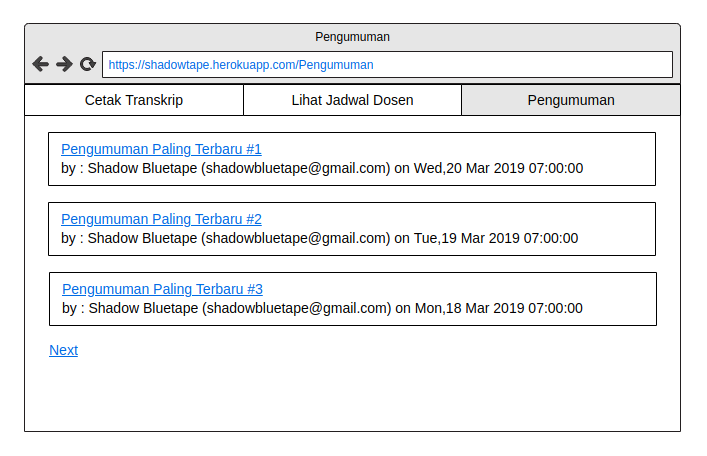
\includegraphics[width=\textwidth]{Mockup-main.png}  
	\caption[\textit{Mockup} antarmuka \textit{main}]{\textit{Mockup} antarmuka \textit{main}} 
	\label{fig:mockup-main} 
\end{figure}

Antarmuka \textit{main} menampilkan daftar pengumuman. Jumlah pengumuman yang ditampilkan di satu halaman dibatasi pada angka tertentu. Di halaman \textit{main} terdapat navigasi \textit{next} dan \textit{prev} untuk menampilkan daftar selanjutnya dan sesudahnya. Gambar~ \ref{fig:mockup-main} menampilkan \textit{mockup} antarmuka \textit{main}.

\subsubsection{read}

\begin{figure}[H]
	\centering  
	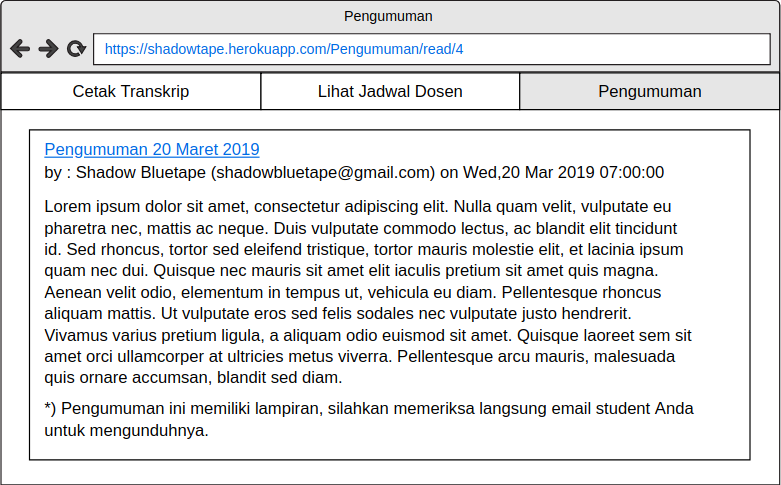
\includegraphics[width=\textwidth]{Mockup-read.png}  
	\caption[\textit{Mockup} antarmuka \textit{read}]{\textit{Mockup} antarmuka \textit{read}} 
	\label{fig:mockup-read} 
\end{figure}

Antarmuka main menampilkan informasi detil dari pengumuman. Apabila pengumuman memiliki lampiran, maka tulisan "*) Pengumuman ini memiliki lampiran, silahkan memeriksa langsung email student Anda untuk mengunduhnya." akan muncul. Jika tidak ada, maka tulisan tersebut tidak akan muncul. Gambar~ \ref{fig:mockup-read} menampilkan \textit{mockup} antarmuka \textit{read}.

\subsection{Perancangan Antarmuka pada \textit{Bot} BlueTape}

\begin{figure}[H]
	\centering  
	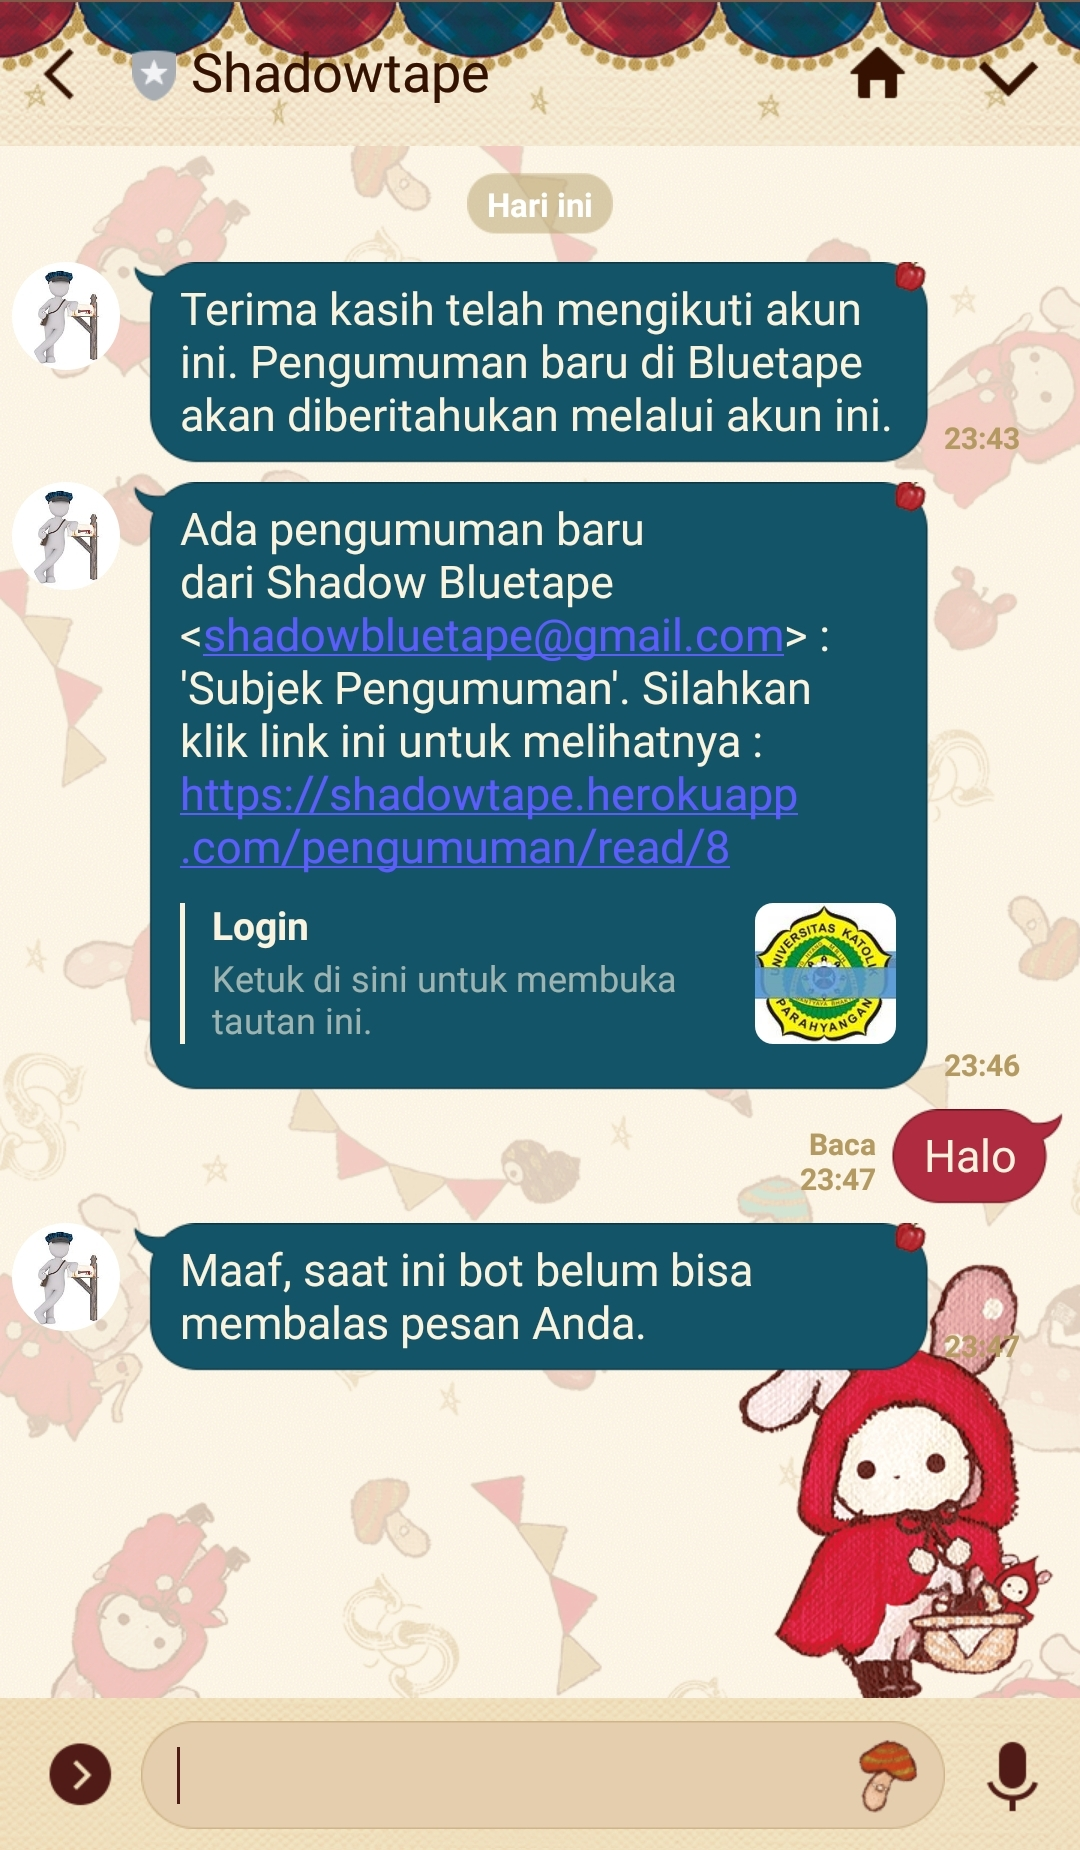
\includegraphics[scale=0.5]{Mockup-bot.jpg}  
	\caption[\textit{Mockup} antarmuka \textit{bot} BlueTape]{\textit{Mockup} antarmuka \textit{bot} BlueTape} 
	\label{fig:mockup-bot} 
\end{figure}

Gambar~\ref{fig:mockup-bot} menampilkan \textit{mockup} antarmuka \textit{bot} BlueTape. \textit{Chat} pertama merupakan pesan yang akan ditampilkan saat \textit{user} baru mengikuti \textit{bot} atau membuka blokir \textit{bot}. \textit{Chat} kedua merupakan contoh pesan yang akan ditampilkan jika ada pengumuman baru yang masuk ke BlueTape. \textit{Chat} terakhir merupakan pesan balasan jika \textit{user} mengirimkan pesan ke \textit{bot} dalam bentuk apapun (teks, \textit{sticker}, gambar, video, dan suara).